\chapter{Instrumentación y Electrónica}
\section{Introducción}

\begin{definition}[LDR]
    La resistencia no lineal, varía en función de la luz que recibe en su superficie. Así, cuando están en oscuridad su resistencia es alta y cuando reciben luz su resistencia disminuye considerablemente.
\end{definition}

\begin{figure}[h!]
\centering
  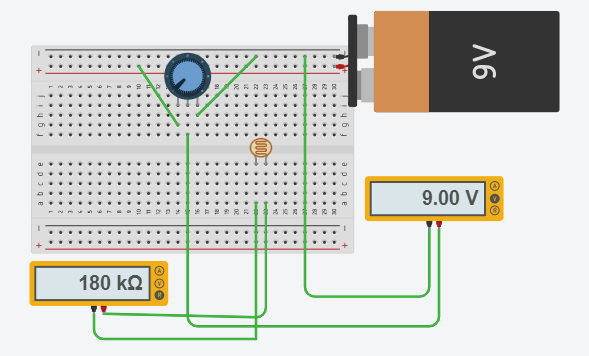
\includegraphics[width=0.5\textwidth]{ie1.png}
  \caption{Ejemplo de un circuito usando fotorresistencia}
  \label{ie1}
\end{figure}

Una fotorresistencia es un componente electrónico cuya resistencia disminuye con el aumento de intensidad de luz incidente. Puede también ser llamado fotorresistor, fotoconductor, célula fotoeléctrica o resistor dependiente de la luz, cuya siglas, LDR, se originan de su nombre en inglés light-dependent resistor.

\begin{figure}[h!]
    \centering
      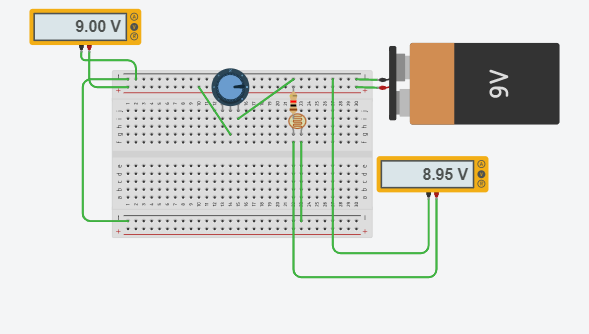
\includegraphics[width=0.5\textwidth]{ie2.png}
      \caption{Uso de una resistencia para monitorear el voltaje}
      \label{ie222}
\end{figure}

\subsubsection{Capacitores}
Se dividen en polarizados o electrolíticos y no polarizados.
\begin{figure}[h!]
  \centering
    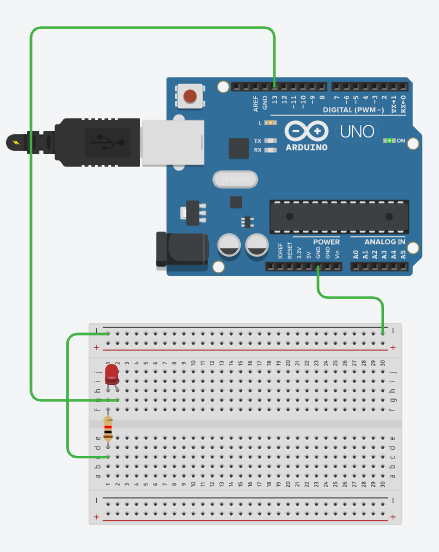
\includegraphics[width=0.5\textwidth]{ie3.png}
    \caption{Uso de arduinos}
    \label{ei3}
\end{figure}
  Éste es el uso de funciones aplicadas a un Arduino 1.
\begin{lstlisting}
  void setup()
  {
    pinMode(LED_BUILTIN, OUTPUT);
  }
  
  void loop()
  {
    digitalWrite(LED_BUILTIN, HIGH);
    delay(1000); // Wait for 1000 millisecond(s)
    digitalWrite(LED_BUILTIN, LOW);
    delay(1000); // Wait for 1000 millisecond(s)
  }
\end{lstlisting}
\begin{itemize}
  \item Botón rojo: Resetear
  \item Pines Analógicos (Verticales), son salidas o entradas
  \item Pines Digitales (Horizontales) Ambos pueden proveer 5V o tierra
\end{itemize}
\begin{figure}[h!]
\centering
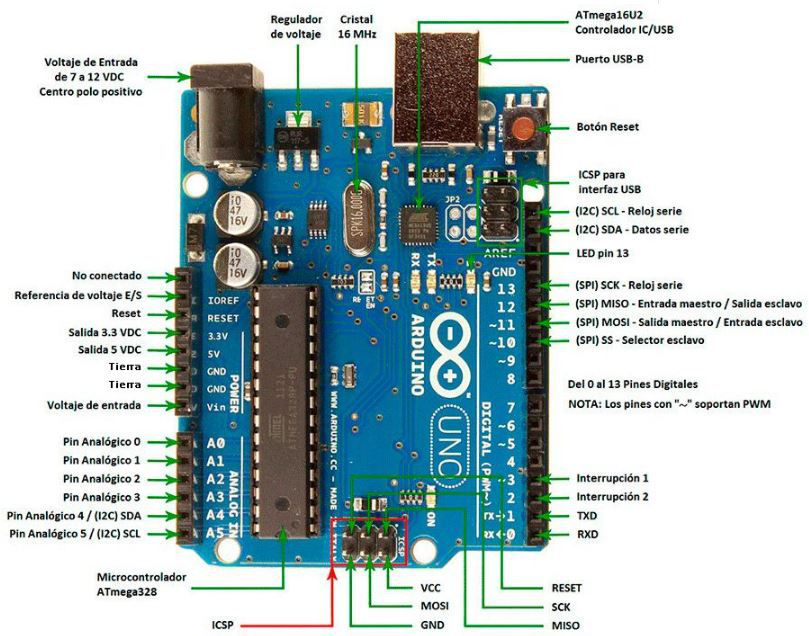
\includegraphics{ie4.png}
\caption{Partes de un Arduino 1}
\label{ie4}
\end{figure}
Para saber si un \texttt{Pin} puede proveer ese voltaje de 5, en programación se pone ``\textbf{HIGH}'' y para tierra ``\textbf{LOW}''. Una salida es ``Output'' y entrada es ``Input'' en lenguaje de Arduino.

\FrameTBStyle{python}
\begin{lstlisting}[style=pythonFrameTB]
  void setup()
  {
      pinMode(6, INPUT);
      pinMode(7, OUTPUT);
  }
  
  void loop()
  {
      digitalWrite(7, HIGH);
      delay(1000);
      digitalWrite(6, LOW);
      delay(1000);
  }
\end{lstlisting}

Genera lo siguiente:
\begin{figure}[h!]
\centering
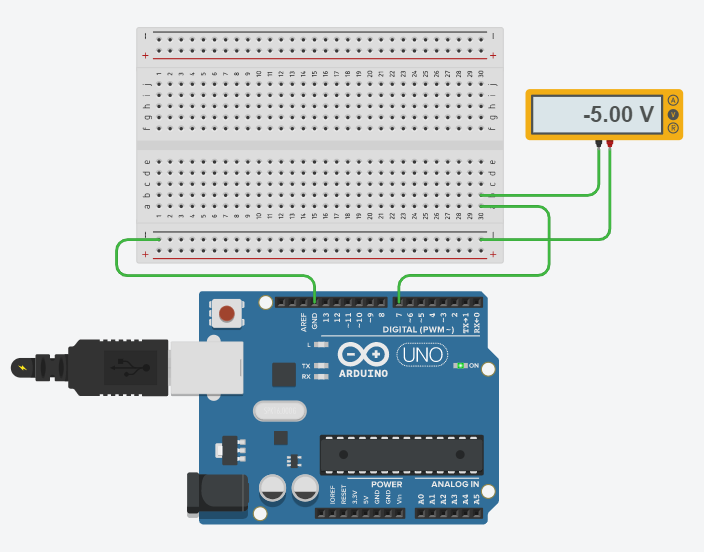
\includegraphics[width=0.5\textwidth]{ie5.png}
\caption{Función de loop en Arduino}
\label{ie5}
\end{figure}
\begin{figure}[h!]
\centering
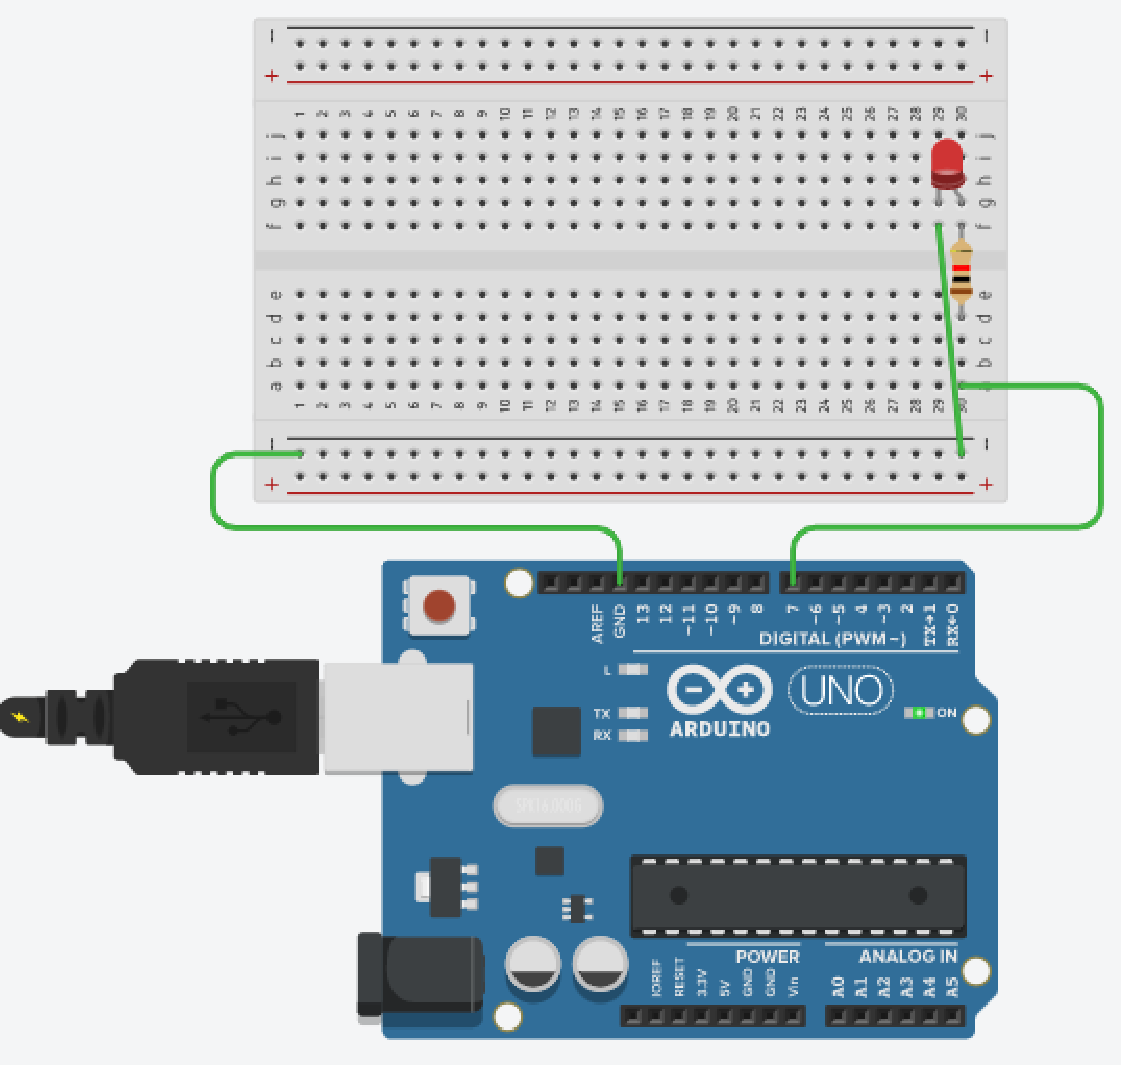
\includegraphics[width=0.5\textwidth]{ie6.pdf}
\caption{Caso donde el tiempo de espera es mayor en el prendido}
\label{ie6}
\end{figure}
\begin{figure}[h!]
\centering
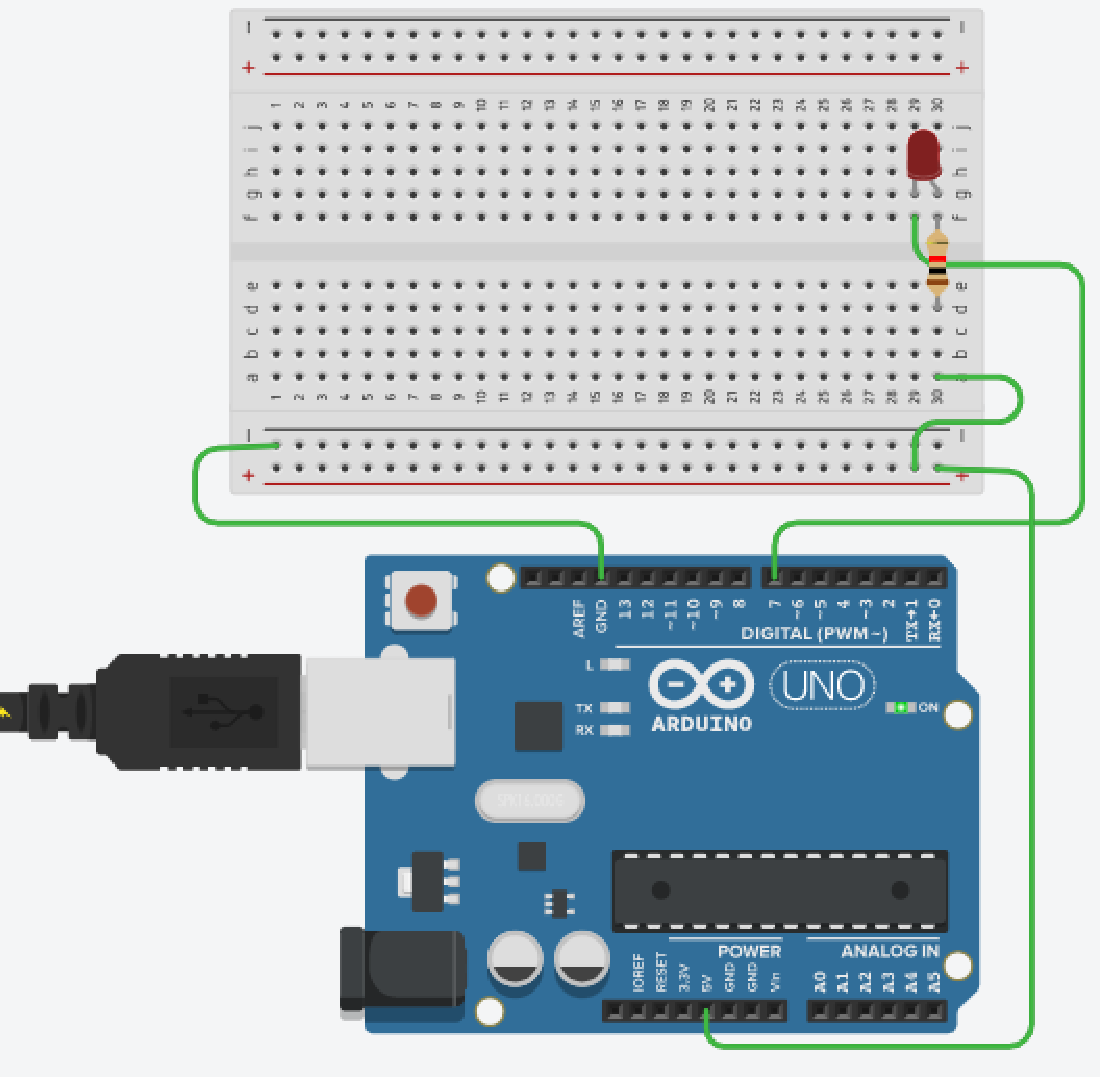
\includegraphics[width=0.5\textwidth]{ie7.pdf}
\caption{Caso donde el tiempo de espera es mayor en el apagado}
\label{ie7}
\end{figure}
Otra aplicación es prender un cátodo con Arduino
\begin{figure}[h!]
\centering
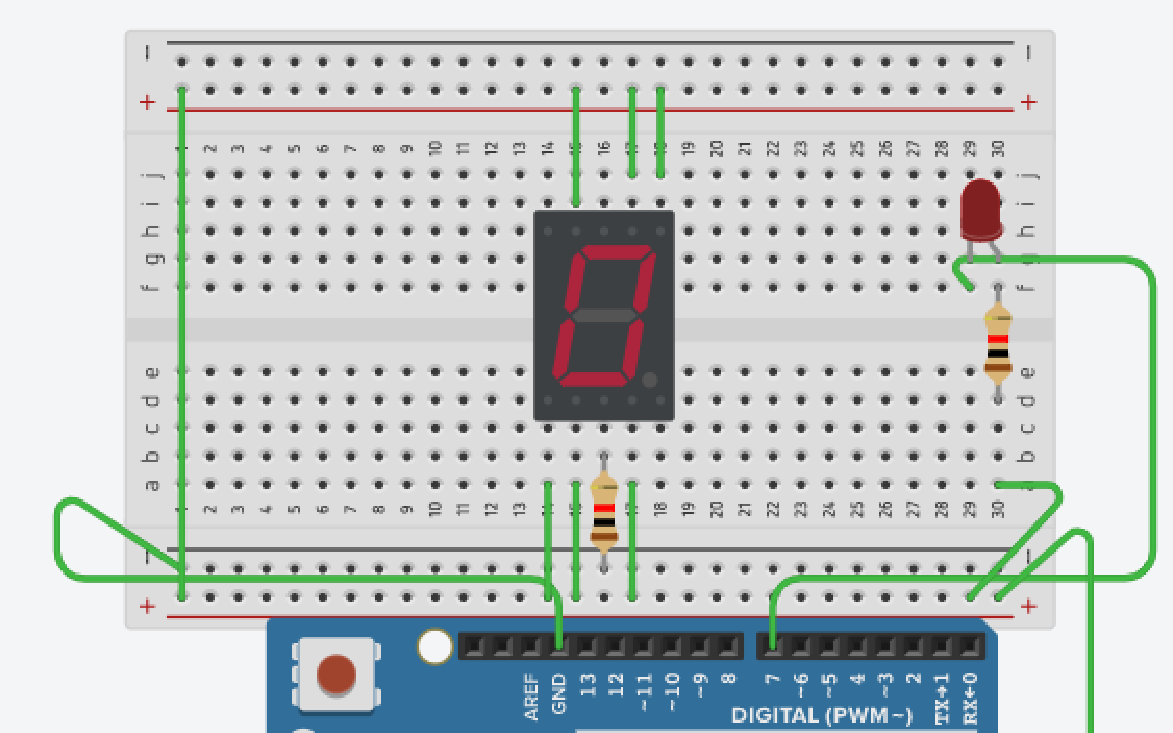
\includegraphics[width=0.5\textwidth]{ie8.pdf}
\caption{número 0 prendido con Arduino y conexiones en el Circuito}
\label{ie8}
\end{figure}

\FrameTBStyle{python}
\begin{lstlisting}[style=pythonFrameTB]
  void setup()
  {
      int i;
      for (i = 1;i <=7;i++)
      pinMode(i, 0);
  }
  
  void loop()
      {
      int i;
      for (i = 1;i <=6;i++)
          digitalWrite(i, 1);
          delay(1000);
      for (i = 1;i <=6;i++)
          digitalWrite(i, 0);
          delay(1000);
          digitalWrite(2, 1);
          digitalWrite(3, 1);
          delay(1000);
          
      };
\end{lstlisting}
\begin{figure}[h!]
\centering
  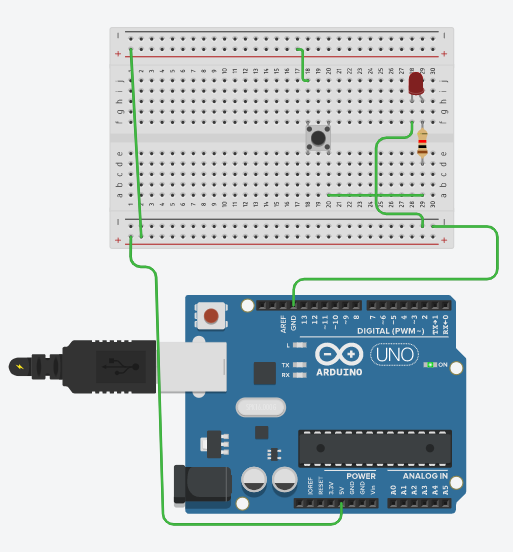
\includegraphics[width=0.5\textwidth]{ie9.png}
  \caption{Arduino para prender un led}
  \label{ie9}
\end{figure}
Si la resistencia es alterada, lo único que cambiará en la simulación es una simulación, mientras más grande sea, más ténue será la luz emitida.
\subsection{Display de 7 segmentos}
Véase que existen dis tipos de display en la figura \ref{ie10}
\begin{figure}[h!]
\centering
  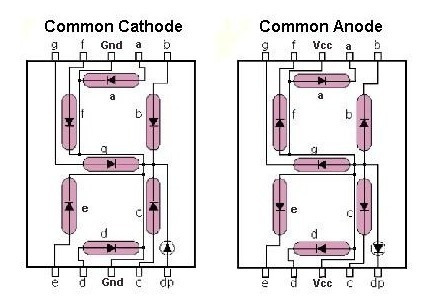
\includegraphics[width=0.5\textwidth]{ie10.jpg}
  \caption{Ánodo y cátodo común}
  \label{ie10}
\end{figure}
Realizaremos el siguiente experimento en TinkerCad:
\begin{figure}[h!]
\centering
  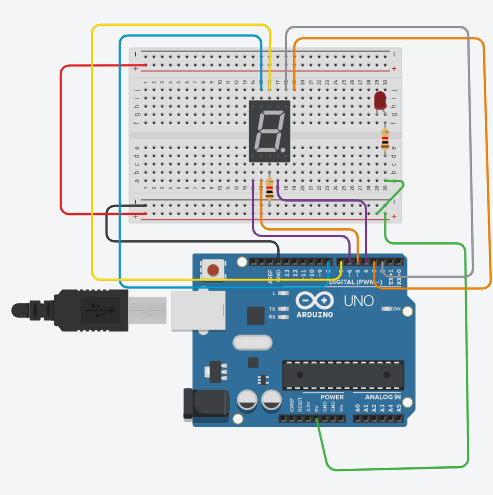
\includegraphics[width=0.5\textwidth]{ie11.png}
  \caption{Display en un circuito}
  \label{ie11}
\end{figure}
\FrameTBStyle{python}
\begin{lstlisting}[style=pythonFrameTB]
    void setup()
    {
      pinMode(2,0); // A
      pinMode(3,0); // B
      pinMode(4,0); // C
      pinMode(5,0); // D
      pinMode(6,0); // E
      pinMode(7,0); // F
      pinMode(8,0); // G
      
    }
    void loop()
        {
            digitalWrite(2, 1);
            delay(1000);
            digitalWrite(3, 0);
            delay(1000);
        digitalWrite(4, 1);
        digitalWrite(5, 1);
        digitalWrite(6, 1);
        digitalWrite(7, 1);
        digitalWrite(8, 1);
        };
  \end{lstlisting}
  \section{Entradas Digitales}

  \FrameTBStyle{c}
  \begin{lstlisting}[style=cFrameTB, gobble=4]
  /*
    Button
  
    Turns on and off a light emitting diode(LED) connected to digital pin 13,
    when pressing a pushbutton attached to pin 2.
  
    The circuit:
    - LED attached from pin 13 to ground through 220 ohm resistor
    - pushbutton attached to pin 2 from +5V
    - 10K resistor attached to pin 2 from ground
  
    - Note: on most Arduinos there is already an LED on the board
      attached to pin 13.
  
    created 2005
    by DojoDave <http://www.0j0.org>
    modified 30 Aug 2011
    by Tom Igoe
  
    This example code is in the public domain.
  
    https://www.arduino.cc/en/Tutorial/BuiltInExamples/Button
  */
  
  // constants won't change. They're used here to set pin numbers:
  const int buttonPin = 2;     // the number of the pushbutton pin
  const int ledPin =  13;      // the number of the LED pin
  
  // variables will change:
  int buttonState = 0;         // variable for reading the pushbutton status
  
  void setup() {
    // initialize the LED pin as an output:
    pinMode(ledPin, OUTPUT);
    // initialize the pushbutton pin as an input:
    pinMode(buttonPin, INPUT);
  }
  
  void loop() {
    // read the state of the pushbutton value:
    buttonState = digitalRead(buttonPin);
  
    // check if the pushbutton is pressed. If it is, the buttonState is HIGH:
    if (buttonState == HIGH) {
      // turn LED on:
      digitalWrite(ledPin, HIGH);
    } else {
      // turn LED off:
      digitalWrite(ledPin, LOW);
    }
  }
  \end{lstlisting}

Produce el siguiente circuito al presionar el botón:
  \begin{figure}[h!]
  \centering
    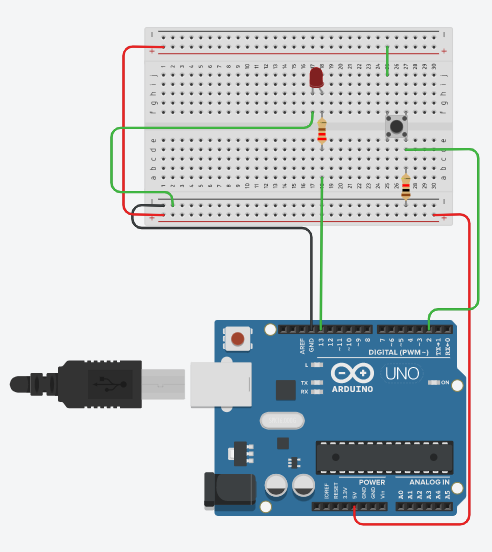
\includegraphics[width=0.5\textwidth]{ie12.png}
    \caption{Como prender un LED con un boton}
    \label{ie12}
\end{figure}
En el siguiente circuito, se encuentra un motor que gira en sentido horario y antihorario cambiando la polaridad con los Switch
que se tienen en la figura \ref{ie13}
\begin{figure}[h!]
\centering
  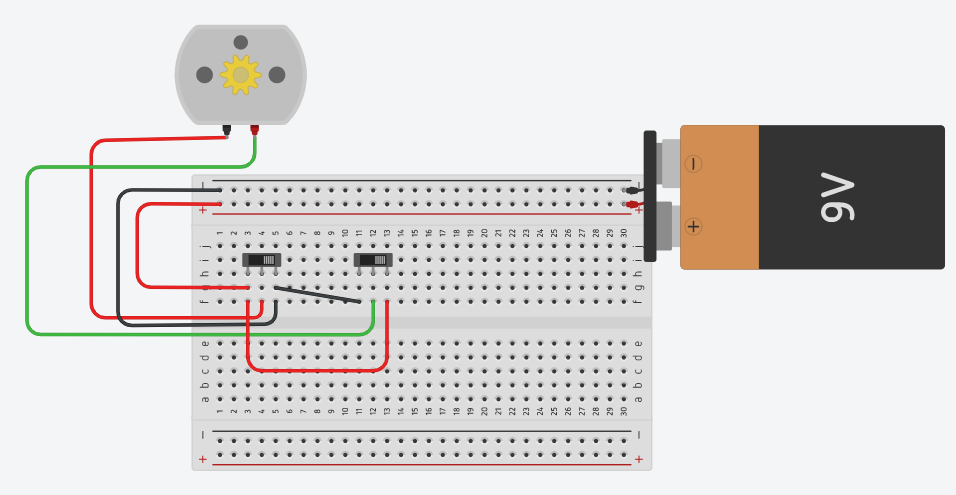
\includegraphics[width=0.5\textwidth]{ie13.png}
  \caption{Motor que gira horario y antihorario dependiendo del switch. El voltaje está relacionada en la velocidad del giro del motor}
  \label{ie13}
\end{figure}
Una fuente de suministro puede crear el mismo efecto con la programación en Arduino:
\begin{figure}[h!]
\centering
  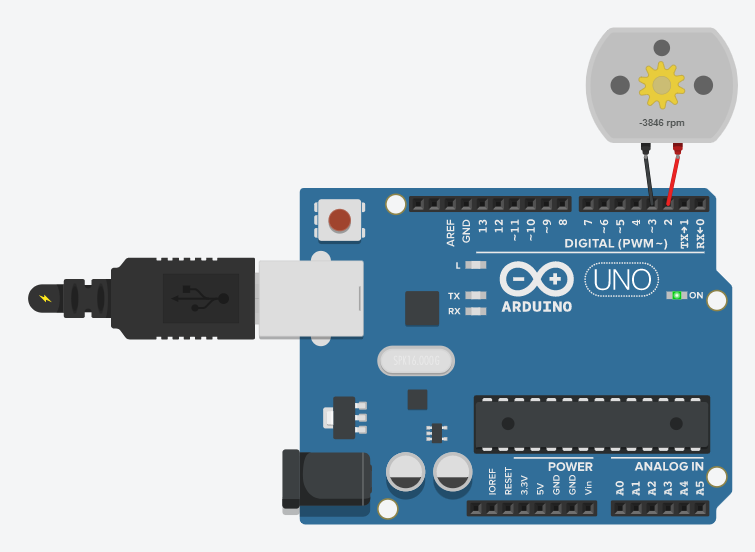
\includegraphics[width=0.5\textwidth]{ie14.png}
  \caption{Cambio de polaridad con programación cada 5 segundos}
  \label{ie14}
\end{figure}
\FrameTBStyle{c}
\begin{lstlisting}[style=cFrameTB, gobble=4]
    void setup()
    {
      pinMode(2, OUTPUT); // Se declaran los pines 2 y 3 como salidas
      pinMode(3, OUTPUT); //Salidas digitales
    }
    
    void loop()
    {
      digitalWrite(2, HIGH);
      digitalWrite(3, LOW);
      delay(5000); // Wait for 1000 millisecond(s)
      digitalWrite(2, LOW);
      digitalWrite(3, HIGH);
      delay(5000); // Wait for 1000 millisecond(s)
    }
\end{lstlisting}

\begin{figure}[h!]
\centering
  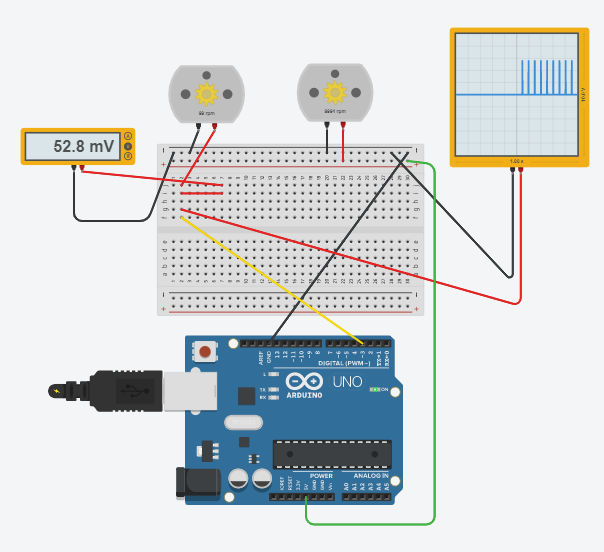
\includegraphics[width=0.5\textwidth]{ie15.png}
  \caption{Cómo conectar dos motores a un Arduino}
  \label{ie15}
\end{figure}
En el siguiente código (Muy simple), se puede controlar el circuito de la figura \ref{ie15}
con la función \textbf{AnalogWrite} y en el Osciloscopio muestra el suministro de voltaje por segundo.
\begin{tikzpicture}[
  scale=\scl,
  controlpanels/.style={yellow!30!brown!20!,rounded corners,draw=black,thick},
  screen/.style={green!50!black!60!,draw=black,thick},
  trace/.style={green!60!yellow!40!, ultra thick},
  smallbutton/.style={white,draw=black, thick},
  axes/.style={thick}]
  \fill[green!30!blue!30!,rounded corners,draw=black,thick](0,0)
    rectangle (27.75,13.25);
  \fill[fill=black!40!,draw=black,thick,rounded corners](0.25,0.25)
    rectangle (27.5,13.00);
  % Screen, centered around the origin then shifted for easy plotting
  \begin{scope}[xshift=7cm,yshift=8cm,samples=150]
    \fill[black!60!,rounded corners,draw=black,thick](-5.3,-4.3)
      rectangle (5.3,4.3);
    \fill[screen] (-5.0,-4.0) rectangle (5.0,4.0);
    \draw[trace] plot(\x,{1+2.4*sin((2.5*\x +1) r)}); % r for radians...
    \draw[trace] plot(\x,{-1+1.25*sin((0.75*\x) r});
    \draw[thin] (-5.0,-4.0) grid (5.0,4.0);
    \draw[axes] (-5,0)--(5,0); % Time axis
    \draw[axes] (0,-4)--(0,4);
    \foreach \i in {-4.8,-4.6,...,4.8} \draw (\i,-0.1)--(\i,0.1);
    \foreach \i in {-3.8,-3.6,...,3.8} \draw (-0.1,\i)--(0.1,\i);
  \end{scope}
  % Feet
  \fill[black!70!,rounded corners,xshift=2cm] (0,-.5) rectangle (2,0);
  \fill[black!70!,rounded corners,xshift=23.75cm] (0,-.5) rectangle (2,0);
  % Lower left panel
  \fill[controlpanels] (0.6,0.5) rectangle (13.5,3.0);
  \path (0.8,0.9) node[scale=\scl,right]{$\mathbf{TeXtronics\,1 - v.1.01}$};
  % Lower right panel
  \fill[controlpanels] (13.7,0.5) rectangle (27.1,6.2);
  %Channels
  % CH I
  \draw[thick] (14.8,1.5) circle (0.7cm);
  \fill[gray,draw=black,thick] (14.8,1.5) circle (0.5cm);
  \fill[white,draw=black,thick] (14.8,1.5) circle (0.3cm);
  \node[scale={1.5*\scl}] at (14.8,2.5) {CH I};
  \draw[thick] (16.2,1.5) circle (0.4cm);
  \fill[black!60!] (16.2,1.5) circle (0.3cm);
  \draw[thick] (16.6,1.5) --(17,1.5)--(17,1.0);
  \draw[thick] (16.7,1.0)--(17.3,1.0);
  \draw[thick] (16.8,0.85)--(17.2,0.85);
  \draw[thick] (16.9,0.70)--(17.1,0.70);
  \draw[thick] (26.0,1.5) circle (0.7cm);
  % CH II
  \fill[gray,draw=black,thick] (26,1.5) circle (0.5cm);
  \fill[white,draw=black,thick] (26,1.5) circle (0.3cm);
  \node[scale={1.5*\scl}] at (26,2.5) {CH II};
  \draw[thick] (24.6,1.5) circle (0.4cm);
  \fill[black!60!] (24.6,1.5) circle (0.3cm);
  \draw[thick] (24.2,1.5) --(23.7,1.5)--(23.7,1.0);
  \draw[thick] (23.4,1.0)--(24.0,1.0);
  \draw[thick] (23.5,0.85)--(23.9,0.85);
  \draw[thick] (23.6,0.70)--(23.8,0.70);
  \draw[thick] (26.0,1.5) circle (0.7cm);
  % Y-pos
  \fill[smallbutton] (14.8,4.9) circle (0.3cm);
  \node[scale={\scl}] at (14.8,5.5) {Y-pos I};
  \fill[smallbutton] (26.0,4.9) circle (0.3cm);
  \node[scale={\scl}] at (26.0,5.5) {Y-pos II};
  % Volt/div the foreach loop draws the two buttons
  \foreach \i / \b in {18/75,22.5/345}{
  %Second parameter of the loop is the angle of the index mark 
  \begin{scope}[xshift=\i cm,yshift=3.8cm,scale=0.85]
    \node[scale=\scl] at (0,2.3) {Volts/Div};
    \node[scale=\scl,black] at (-1,-2.4) {V};
    \node[scale=\scl,blue]  at (1,-2.4) {mV};
    \clip[rounded corners] (-2,-2) rectangle (2,2);
    \fill[black!30!,rounded corners,draw=black,thick] (-2,-2)
      rectangle (2,2);
    \fill[blue!50!black!20!,draw=black,thick]
      (30:1.1)--(30:3)--(3,-3)--(-90:3)--(-90:1.1) arc (-90:30:1.1);
    \draw[very thick,rounded corners](-2,-2) rectangle (2,2);
    \draw[thick] (0,0) circle (1.0);
    \foreach \i in {0,30,...,330}
      \draw[thick] (\i:1.2)--(\i:2.5);
    \foreach \i/\j in {15/50,45/.1,75/.2,105/.5,135/1,165/2,195/5,225/10,
      255/20,285/5,315/10,345/20} \node[scale=\scl,black] at (\i:1.7) {\j};
    \fill[blue!30!black!60!,draw=black,thick] (0,0) circle (0.8cm);
    % Here you set the right Volts/Div button
    \draw[ultra thick,red] (\b:0.3)--(\b:1.2);
  \end{scope}}
% Upper right panel
  \fill[controlpanels] (13.7,6.5) rectangle (27.1,12.75);
  %On-Off button
  \draw[rounded corners,thick,blue] (13.9,10.5) rectangle (15.9,12.5);
  \fill[fill=red,draw=black,thick,rounded corners] (14.4,10.8) rectangle (15.3,11.2);
  \node[scale=\scl] at (14.8,12) {\textbf{Power}};
  \node[scale=\scl] at (14.8,11.5) {\textbf{On/Off}};
  % Focus-Intensity buttons
  \draw[rounded corners,thick,blue] (13.9,7.0) rectangle (15.9,10.0);
  \fill[smallbutton] (14.9,7.5) circle (0.3cm);
  \node[scale=\scl] at (14.9,8.2) {\textbf{Focus}};
  \fill[smallbutton] (14.9,9) circle (0.3cm);
  \node[scale=\scl] at (14.9,9.6) {\textbf{Intens}};
  % X-pos
  \fill[smallbutton] (24.5,9.9) circle (0.3cm);
  \node[scale={\scl}] at (24.5,10.5) {X-pos};
  % Time/Div
  \begin{scope}[xshift=21cm,yshift=9.5cm,scale=1]
    \node[scale={1.25*\scl}]  at (0,2.4) {Time/Div};
    \clip[rounded corners] (-2.2,-2) rectangle (2.2,2);
    \fill[black!30!,rounded corners,draw=black,thick] (-2.2,-2) rectangle (2.2,2);
    \fill[blue!50!black!20!,draw=black,thick]
      (45:1.1)--(45:3)--(3,-3)--(-90:3)--(-90:1.1) arc (-90:45:1.1);
    \fill[green!50!black!40!,draw=black,thick]
      (45:1.1)--(45:3) arc(45:207:3) --(207:1.1) arc (207:45:1.1);
    \draw[very thick,rounded corners](-2.2,-2) rectangle (2.2,2);
    \node[scale={1.25*\scl}] at (-1.6,-1.6) {$s$};
    \node[scale={1.25*\scl}] at (1.6,-1.6) {$\mu{}\,s$};
    \node[scale={1.25*\scl}] at (-1.6,1.6) {$m\,s$};
    \draw[thick] (0,0) circle (1.0);
    \foreach \i in {-72,-54,...,262} \draw[thick] (\i:1.15)--(\i:1.35);
    \foreach \i/\j in {-72/.5,-54/1,-36/2,-18/5,0/10,18/20,36/50,54/.1,72/.2,90/.5,
      108/1,126/2,144/5,162/10,180/20,198/50,216/.1,234/.2,252/.5}
      \node[scale=\scl,black] at (\i:1.7){\j};
    \fill[blue!30!black!60!,draw=black,thick] (0,0) circle (0.8cm);
    % Here you set the Time/Div button
    \draw[ultra thick,red] (-18:0.3)--(-18:1.2);	
    % X-pos
  \end{scope}
\end{tikzpicture}
\FrameTBStyle{c}
\begin{lstlisting}[style=cFrameTB, gobble=4]
void setup()
{
  pinMode(3, OUTPUT); //Salidas digitales
}

void loop()
{
  int i;
  analogWrite(3,5); // Se escribe en el pin 3, el valor 5.
  delay(1000);
}
\end{lstlisting}
\subsection{PWM}

La modulación de ancho de pulso, o PWM, es una técnica para obtener resultados analógicos con medios digitales. El control digital se utiliza para crear una onda cuadrada, una señal que cambia entre encendido y apagado. Este patrón de encendido y apagado puede simular voltajes entre el Vcc completo de la placa (p. ej., 5 V en Uno, 3,3 V en una placa MKR) y apagado (0 voltios) al cambiar la parte del tiempo que pasa la señal en comparación con el tiempo que la señal pasa apagada. La duración de "a tiempo" se denomina ancho de pulso. Para obtener valores analógicos variables, cambia o modula ese ancho de pulso. Si repite este patrón de encendido y apagado lo suficientemente rápido con un LED, por ejemplo, el resultado es como si la señal fuera un voltaje constante entre 0 y Vcc que controla el brillo del LED.

En el siguiente gráfico, las líneas verdes representan un período de tiempo regular. 

Esta duración o período es el inverso de la frecuencia PWM. En otras palabras, con la frecuencia PWM de Arduino a unos 500 Hz, las líneas verdes medirían 2 milisegundos cada una. Una llamada a \texttt{analogWrite()} está en una escala de 0 a 255, de modo que analogWrite(255) solicita un ciclo de trabajo del 100\% (siempre activo), y analogWrite(127) es un ciclo de trabajo del 50\% (en la mitad del tiempo) para ejemplo.
\begin{figure}[h!]
\centering
  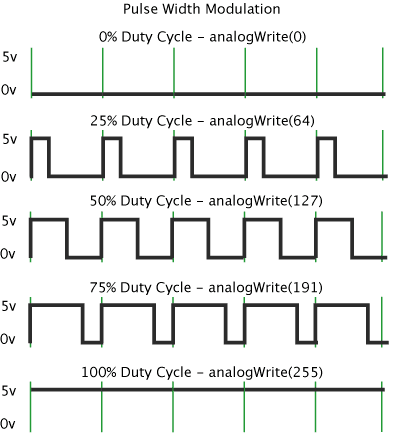
\includegraphics[width=0.5\textwidth]{ie16.png}
  \caption{salida analógica}
  \label{ie16}
\end{figure}

\FrameTBStyle{c}
\begin{lstlisting}[style=cFrameTB, gobble=4]
void setup()
{
  pinMode(3, OUTPUT); //Salidas digitales
}

void loop()
{
  int i;
  for(i=0;i<255;i++){
  analogWrite(3,i);
    delay(500);}
}
\end{lstlisting}


\subsubsection{Potenciómetro}

\begin{figure}[h!]
\centering
  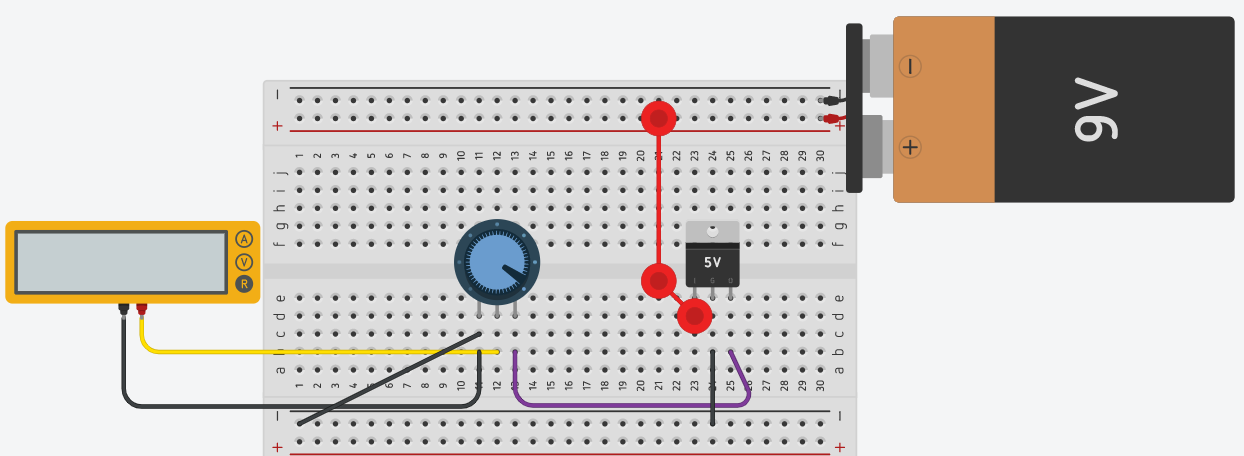
\includegraphics[width=0.5\textwidth]{ie17.png}
  \caption{Uso del potenciómetro}
  \label{ie17}
\end{figure}
\begin{figure}[h!]
  \centering
    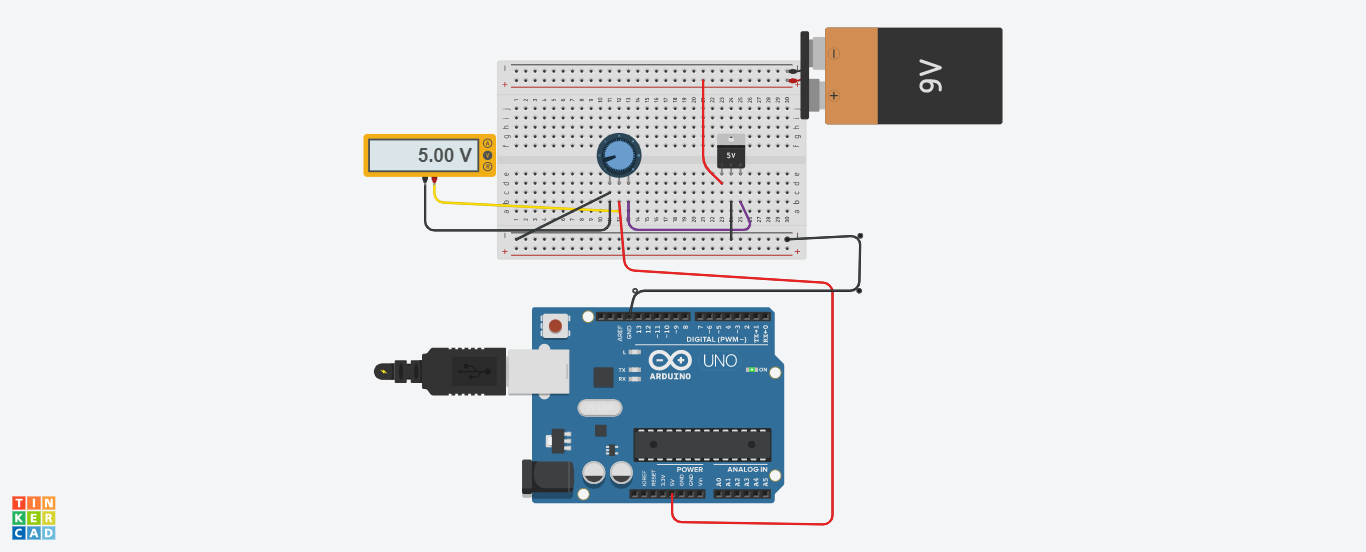
\includegraphics[width=0.5\textwidth]{ie18.png}
    \caption{Regulador de voltaje con arduino}
    \label{ie18}
  \end{figure}
  
\FrameTBStyle{c}
\begin{lstlisting}[style=cFrameTB, gobble=4]
  const int analogInPin= A0;
  int sensorValue =0;
  
  void setup()
  {
    Serial.begin(9600);
  }
  
  void loop()
  {
    sensorValue= analogRead(analogInPin);
    Serial.print("sensor = ");
    Serial.println(sensorValue);
    delay(2);
  }
\end{lstlisting}
\subsection{Cristal líquido}
\FrameTBStyle{c}
\begin{lstlisting}[style=cFrameTB, gobble=4]
/*
  LiquidCrystal Library - scrollDisplayLeft() and scrollDisplayRight()

 Demonstrates the use a 16x2 LCD display.  The LiquidCrystal
 library works with all LCD displays that are compatible with the
 Hitachi HD44780 driver. There are many of them out there, and you
 can usually tell them by the 16-pin interface.

 This sketch prints "Hello World!" to the LCD and uses the
 scrollDisplayLeft() and scrollDisplayRight() methods to scroll
 the text.

  The circuit:
 * LCD RS pin to digital pin 12
 * LCD Enable pin to digital pin 11
 * LCD D4 pin to digital pin 5
 * LCD D5 pin to digital pin 4
 * LCD D6 pin to digital pin 3
 * LCD D7 pin to digital pin 2
 * LCD R/W pin to ground
 * 10K resistor:
 * ends to +5V and ground
 * wiper to LCD VO pin (pin 3)

 Library originally added 18 Apr 2008
 by David A. Mellis
 library modified 5 Jul 2009
 by Limor Fried (http://www.ladyada.net)
 example added 9 Jul 2009
 by Tom Igoe
 modified 22 Nov 2010
 by Tom Igoe
 modified 7 Nov 2016
 by Arturo Guadalupi

 This example code is in the public domain.

 http://www.arduino.cc/en/Tutorial/LiquidCrystalScroll

*/

// include the library code:
#include <LiquidCrystal.h>

// initialize the library by associating any needed LCD interface pin
// with the arduino pin number it is connected to
const int rs = 12, en = 11, d4 = 5, d5 = 4, d6 = 3, d7 = 2;
LiquidCrystal lcd(rs, en, d4, d5, d6, d7);

void setup() {
  // set up the LCD's number of columns and rows:
  lcd.begin(16, 2);
  // Print a message to the LCD.
  lcd.print("Hola Mundo");
  delay(1000);
}
void loop () {
  int i;
  char c;
  	for (i=0;i<=255;i++)
    {
      c=i;
      lcd.setCursor(0,1); lcd.print(i);lcd.print(" ");lcd.print(c);
      delay(500);
    }
}
\end{lstlisting}
\begin{figure}[h!]
\centering
  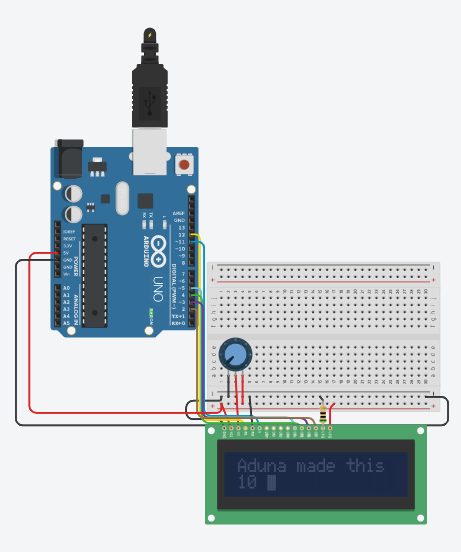
\includegraphics[width=0.5\textwidth]{ie19.png}
  \caption{Circuito para prender una pantalla led}
  \label{ie19}
\end{figure}

De éste circuito, se pretende encontrar los datos de temperatura y mostrarlos en la pantalla, de manera que modificaremos el circuito y la programación de la siguiente manera:
\FrameTBStyle{c}
\begin{lstlisting}[style=cFrameTB, gobble=4]
    #include <LiquidCrystal.h>
    float media(float datos[], int n);
    const int rs = 12, en = 11, d4 = 5, d5 = 4, d6 = 3, d7 = 2;
    LiquidCrystal lcd(rs, en, d4, d5, d6, d7);
    const int analogInPin = A0;
    int sensor=0;
    //Se declaran los pines a los que iran conectados los leds.
    int LED_AZUL=8;
    int LED_VERDE=9;
    int LED_ROJO=10;
    
    
    void setup() 
    {
        lcd.begin(16,2);
        Serial.begin(9600);
    //Se declaran los pines del 8 a 10 como salidas
        pinMode(LED_AZUL,OUTPUT);  
        pinMode(LED_VERDE,OUTPUT);
        pinMode(LED_ROJO,OUTPUT);
    }
    
    
    void loop() {
      float sensor;
      float temperatura;
      char c=223;
      float T[31];
      // Se obtiene 30 lecturas en el ciclo for 
      int i,n=30;
      int senal;
      for (i=1;i<=30;i++){
        sensor=analogRead(analogInPin);
     temperatura = (sensor * 500.0/ 1023.0) - 50.0;
     //Serial.print("Lectura ");Serial.print(i);Serial.print(" ");Serial.println(temperatura);
     delay(5);
     T[i]=temperatura;
     delay(10);
      }
    
     Serial.print("_______________");
     temperatura=media(T,n);
     lcd.clear();
     lcd.print("Tem:"); lcd.print(temperatura);lcd.print(" ");lcd.print(c);lcd.print("C");
     Serial.print("sensor =");
     Serial.print(temperatura);
     Serial.print(c);Serial.println(" C");
      if (temperatura<10.0)
      {
          senal =-1;
              digitalWrite(LED_AZUL,HIGH);
              digitalWrite(LED_VERDE,LOW);
              digitalWrite(LED_ROJO,LOW);
      }
      if (temperatura >=10.0 && temperatura<=25.5 )
      {
          senal =0;
            digitalWrite(LED_AZUL,LOW);
              digitalWrite(LED_VERDE,HIGH);
              digitalWrite(LED_ROJO,LOW);
      }
          if (temperatura>25.5)
      {
          senal =1;
            digitalWrite(LED_AZUL,LOW);
              digitalWrite(LED_VERDE,LOW);
              digitalWrite(LED_ROJO,HIGH);
      }
         Serial.print("Valor de la senal:");Serial.println(senal);
     delay(500);
    }
    
    
    
    
    float media(float datos[],int n)
    {
    float suma,media;
    int i;
    suma=0.0;
    for(i=1;i<=n;i++)
         suma=suma+datos[i];
         media=suma/n;
    return(media);
    }
\end{lstlisting}
\begin{figure}[h!]
    \centering
      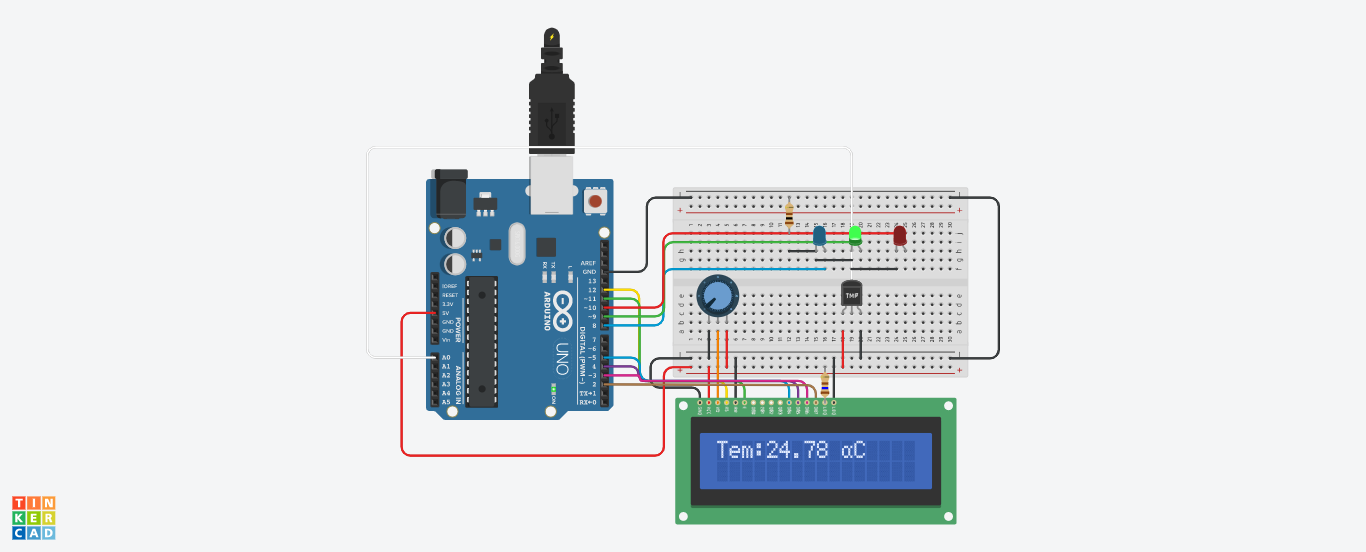
\includegraphics[width=0.5\textwidth]{ie20.png}
      \caption{Circuito que imprime la humedad atmosférica, y prende una luz led dependiendo un rango de temperatura}
      \label{ie20}
\end{figure}
\FrameTBStyle{c}
\begin{lstlisting}[style=cFrameTB, gobble=4]
// include the library code:
#include <LiquidCrystal.h>

// initialize the library by associating any needed LCD interface pin
// with the arduino pin number it is connected to
const int rs = 12, en = 11, d4 = 5, d5 = 4, d6 = 3, d7 = 2;
LiquidCrystal lcd(rs, en, d4, d5, d6, d7);
int Sensor_HS=A0;// Entrada analogica
  
void setup() {
  // set up the LCD's number of columns and rows:
  lcd.begin(16, 2);
  // initialize serial communications at 9600 bps:
  Serial.begin(9600);
  
}

void loop() {
  int Valor_sensor;
  Valor_sensor = analogRead(Sensor_HS);
  lcd.print("Valor:");
  lcd.print(Valor_sensor);
  Serial.println(Valor_sensor);
  delay(500);
  lcd.clear();
}
\end{lstlisting}
% \begin{figure}[h!]
%     \centering
%       \includegraphics[width=0.5\textwidth]{ie21.png}
%       \caption{Expresar la humedad del suelo con un sensor}
%       \label{ie21}
% \end{figure}









































